
\begin{figure}[h]        
    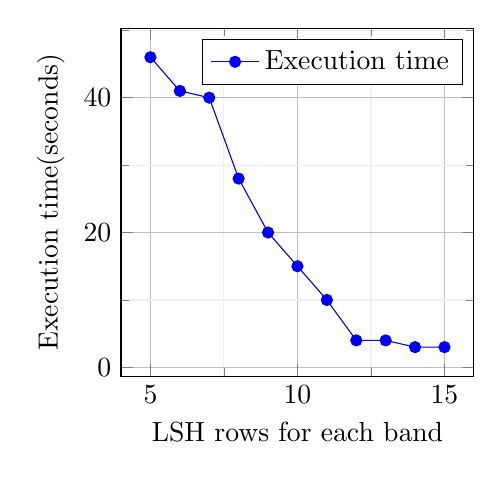
\begin{tikzpicture}
    \begin{axis}[
        xlabel=LSH rows for each band,
        ylabel=Execution time(seconds),
        height=6cm,
        width = 0.5*\textwidth,
        grid = both,
        minor tick num = 1,
        major grid style = {lightgray},
        minor grid style = {lightgray!25},
        legend cell align = {left},
        legend pos = north east
    ]
    
    \addplot[color=blue,mark=*] coordinates {
        (5, 46)
        (6, 41)
        (7, 40)
        (8, 28)
        (9, 20)
        (10, 15)
        (11, 10)
        (12, 4)
        (13, 4)
        (14, 3)
        (15, 3)
    };
    
    \legend{Execution time}
    \end{axis}
    \end{tikzpicture}
    
    \caption{\normalfont The time required to search for the most similar query decreases as the size of each band increases.}
    \label{fig:rows_per_band_time}
\end{figure}
